
%%%%%%%%%%%%%%%%%%%%%%%%%%%%%%%%%%%%%%%%%%%%%%%%%%%%%%%%%%%%%%%%%%%%%%
\begin{frame}[fragile]\frametitle{}
\begin{center}
{\Large Graph}
\end{center}

\end{frame}


\begin{frame}
	\frametitle{A Graph}

	\begin{columns}
		\column{0.405\textwidth}
		\begin{tikzpicture}[scale=0.8, transform shape]
	\begin{scope}[every node/.style={circle,thick,draw,onslide=<2>{draw=red}}]
    \node (A) at (0,0) {A};
    \node (B) at (0,3) {B};
    \node (C) at (2.5,4) {C};
    \node (D) at (2.5,1) {D};
    \node (E) at (2.5,-3) {E};
    \node (F) at (5,3) {F} ;
\end{scope}

\begin{scope}[>={Stealth},
              every node/.style={fill=white,circle},
							every edge/.style={very thick, draw=black,onslide=<3>{draw=red}}]
    \path (A) edge (B);
    \path (B) edge (C);
    \path (A) edge (D);
    \path (D) edge (C);
    \path (A) edge (E);
    \path (D) edge (E);
    \path (D) edge (F);
    \path (C) edge (F);
    \path (E) edge (F); 
    \path (B) edge[bend right=60] (E); 
\end{scope}
\end{tikzpicture}

		\column{0.605\textwidth}
		\begin{itemize}
			\item A graph is just a bunch of circles and lines.
				\pause
			\item These circles are called \alert{vertices} (or \alert{nodes}).
				\pause
			\item These lines are called \alert{edges} (or \alert{connections}).
				\pause
			\item In this form the graph is called \textit{undirected} and \textit{unweighted}.
		\end{itemize}
	\end{columns}
\end{frame}

\begin{frame}
	\frametitle{Directed Graphs}
	
	\begin{columns}
		\column{0.405\textwidth}
		\alt<2>{
			\begin{tikzpicture}[scale=0.8, transform shape]
\begin{scope}[every node/.style={circle,thick,draw}]
    \node (A) at (0,0) {A};
    \node (B) at (0,3) {B};
    \node (C) at (2.5,4) {C};
    \node (D) at (2.5,1) {D};
    \node (E) at (2.5,-3) {E};
    \node (F) at (5,3) {F} ;
\end{scope}

\begin{scope}[>={Stealth[black]},
              every node/.style={fill=white,circle},
              every edge/.style={draw=black,very thick}]
    \path [->] (A) edge node {$5$} (B);
    \path [->] (B) edge node {$3$} (C);
    \path [->] (A) edge node {$4$} (D);
    \path [->] (D) edge node {$3$} (C);
    \path [->] (A) edge node {$3$} (E);
    \path [->] (D) edge node {$3$} (E);
    \path [->] (D) edge node {$3$} (F);
    \path [->] (C) edge node {$5$} (F);
    \path [->] (E) edge node {$8$} (F); 
    \path [->] (B) edge[bend right=60] node {$1$} (E); 
\end{scope}
\end{tikzpicture}

			}{
			\begin{tikzpicture}[scale=0.8, transform shape]
	\begin{scope}[every node/.style={circle,thick,draw}]
    \node (A) at (0,0) {A};
    \node (B) at (0,3) {B};
    \node (C) at (2.5,4) {C};
    \node (D) at (2.5,1) {D};
    \node (E) at (2.5,-3) {E};
    \node (F) at (5,3) {F} ;
\end{scope}

\begin{scope}[>={Stealth},
              every node/.style={fill=white,circle},
							every edge/.style={draw=black,very thick}]
							\path[->] (A) edge (B);
							\path[->] (B) edge (C);
							\path[->] (A) edge (D);
							\path[->] (D) edge (C);
							\path[->] (A) edge (E);
							\path[->] (D) edge (E);
							\path[->] (D) edge (F);
							\path[->] (C) edge (F);
							\path[->] (E) edge (F); 
							\path[->] (B) edge[bend right=60] (E); 
\end{scope}
\end{tikzpicture}

		}
		\column{0.605\textwidth}
		\begin{itemize}
			\item Edges can also have a direction.
			\item In which case we call it a \textit{directed} graph.
				\pause
			\item Furthermore they can have weights.
			\item In which case we call it a \textit{weighted} graph.
		\end{itemize}
	\end{columns}
\end{frame}

\begin{frame}
	\frametitle{Let's formalise!}

		\begin{block}{A formal definition of a graph}
			\begin{itemize}
				\item A graph $G=(V,E)$, where:
					\begin{itemize}
						\item $V$ is a set of vertices,
						\item $E$ is a set of edges, where every edge has two \textit{endpoints}.
					\end{itemize}
					\pause
				\item If the graph is \textit{weighted} then there is a function $w: E \to \mathbb{R}$ which maps every edge to
					a weight.
					\pause
					\begin{itemize}
						\item In most cases we will restrict ourselves to functions $w: E \to \mathbb{N}$, i.e. non-negative integer weights.
					\end{itemize}
					\pause
				\item Depending on direction:
					\begin{itemize}
					\pause
						\item If the graph is \textit{directed} then every edge $e = (u,v)$ with $u,v \in V$. In this case we call
							$u$ the \textit{origin} and $v$ the \textit{destination}
					\pause
				\item If the graph is \textit{undirected} then every edge $e = \{u,v\}$ with $u,v \in V$.\footnote{Unfortunately
						in many textbooks/papers/slides people also use $e=(u,v)$ for undirected edges, but just remark they are
					undirected.}
					\end{itemize}
			\end{itemize}
		\end{block}	
\end{frame}

\begin{frame}
	\frametitle{Let's draw}

	\begin{block}{Just like Toothless}
		Draw the following graph:
		\begin{itemize}
			\item $V = \{A,B,C,D,E,F\}$\\
			\item	$E = \{
			\{A, B\},
			\{A, D\},
			\{D, C\},
			\{B, F\},
			\{B, E\},$\\$
			\{E, D\},
			\{E, F\},
			\{C, F\},
			(A,C),
			(C,A),
			(D,B),
			(B,C)
		\}$\\
	\item $w(\{E,D\}) = 8$, $w((A,C)) = 2$, $w(\{C,F\}) = 5$, $w(\{E,B\}) = 2$, $w((C,A)) = 8$.
		For all other edges $e$, $w(e) = 1$.
		\end{itemize}
	\end{block}
\end{frame}

\begin{frame}
	\frametitle{Properties of vertices}
		
	\begin{columns}
		\column{0.405\textwidth}
			\begin{tikzpicture}[scale=0.8, transform shape]
	\begin{scope}[every node/.style={circle,thick,draw}]
		\node[onslide=<2-3>{draw=red}] (A) at (0,0) {A};
    \node (B) at (0,3) {B};
    \node[onslide=<4-5>{draw=red}] (C) at (2.5,4) {C};
		\node[onslide=<2>{draw=red}] (D) at (2.5,1) {D};
    \node (E) at (2.5,-3) {E};
    \node (F) at (5,3) {F} ;
\end{scope}

\begin{scope}[>={Stealth},
              every node/.style={fill=white,circle},
							every edge/.style={draw=black,very thick}]
							\path[onslide=<4->{->}] (A) edge[onslide=<3>{draw=red}] (B);
							\path[onslide=<4->{->}] (B) edge[onslide=<4>{draw=red}] (C);
							\path[onslide=<4->{->}] (A) edge[onslide=<3>{draw=red}] (D);
							\path[onslide=<4->{->}] (D) edge[onslide=<4>{draw=red}] (C);
							\path[onslide=<4->{->}] (A) edge[onslide=<3>{draw=red}] (E);
							\path[onslide=<4->{->}] (D) edge (E);
							\path[onslide=<4->{->}] (D) edge (F);
							\path[onslide=<4->{->}] (C) edge[onslide=<5>{draw=red}] (F);
							\path[onslide=<4->{->}] (E) edge (F); 
							\path[onslide=<4->{->}] (B) edge[bend right=60] (E); 
\end{scope}
\end{tikzpicture}

		\column{0.605\textwidth}
		Vertices also have some properties:
		\pause
		\begin{itemize}
			\item Two vertices are \alert{adjacent} if there is an edge between them.
			\item We also call these \alert{neighbouring} vertices.
				\pause
			\item Every vertex has a set of \alert{incident} edges, namely those connected to it.
				\pause
			\item If the graph is directed, we can split this into:
				\begin{itemize}
					\item \alert{incoming} edges.
						\pause
					\item \alert{outgoing} edges.
				\end{itemize}
		\end{itemize}
	\end{columns}
\end{frame}

\begin{frame}
	\frametitle{More formalisation}
	\begin{block}{Properties of vertices}
		\begin{itemize}
			\item Two vertices $u,v \in V$ are adjacent, or neighbours, iff $\exists e \in E$ s.t. $e=(u,v)$.
				\pause
			\item The set of neighbours of $u$ is all of the nodes $v \in V$ that are neighbours of $u$.
				\pause
			\item An edge $e$ is incident to a vertex $v$ if $e=(u,v)$ or $e = (v,u)$ for some $u \in V$.
				\pause
			\item The \alert{degree} of a vertex $v$ is the number of incident edges to $v$, so $\mathit{deg}: V \to \mathbb{N}$.
				\pause
			\item For a directed graph, we define $\mathit{indeg}: V \to \mathbb{N}$ and $\mathit{outdeg}: V \to \mathbb{N}$,
				such that:
				\pause
				\begin{itemize}
					\item $\mathit{indeg}(v) = | \{u \mid (u,v) \in E\}|$
					\item $\mathit{outdeg}(v) = | \{u \mid (v,u) \in E\}|$
						\pause
					\item This means that: $\mathit{indeg}(v) + \mathit{outdeg}(v) = \mathit{deg}(v)$.
				\end{itemize}
		\end{itemize}
	\end{block}	
\end{frame}

\begin{frame}
	\frametitle{Lets check again}
	\begin{columns}
		\column{0.405\textwidth}
			\begin{tikzpicture}[scale=0.8, transform shape]
	\begin{scope}[every node/.style={circle,thick,draw}]
		\node[] (A) at (0,0) {A};
    \node (B) at (0,3) {B};
    \node[] (C) at (2.5,4) {C};
		\node[] (D) at (2.5,1) {D};
    \node (E) at (2.5,-3) {E};
    \node (F) at (5,3) {F} ;
\end{scope}

\begin{scope}[>={Stealth[black]},
              every node/.style={fill=white,circle},
							every edge/.style={draw=black,very thick}]
							\path[->] (A) edge (B);
							\path[->] (B) edge (C);
							\path[->] (A) edge (D);
							\path[->] (D) edge (C);
							\path[->] (A) edge (E);
							\path[->] (D) edge (E);
							\path[->] (D) edge (F);
							\path[->] (C) edge (F);
							\path[->] (E) edge (F); 
							\path[->] (B) edge[bend right=60] (E); 
\end{scope}
\end{tikzpicture}

		\column{0.605\textwidth}
	\begin{block}{What dos the following result in?}
	\pause
		$\mathit{outdeg}(D) + \mathit{indeg}(C) + \sum\limits_{v\in \{v \in V \mid (B,v) \in E\}} \mathit{deg}(v) = $
		\begin{enumerate}[A.]
			\item 4
			\item 8
			\item 12
			\item 16
			\item I don't know.
		\end{enumerate}
	\end{block}
	\pause
	\begin{block}{If I did my math right...}
		3 leaving $D$, 2 entering $C$ and the degrees of C and E (3 and 4) makes 12.
	\end{block}
	\end{columns}
\end{frame}

\begin{frame}
	\frametitle{There are extensions/special cases}
	\begin{columns}
		\column{0.405\textwidth}
			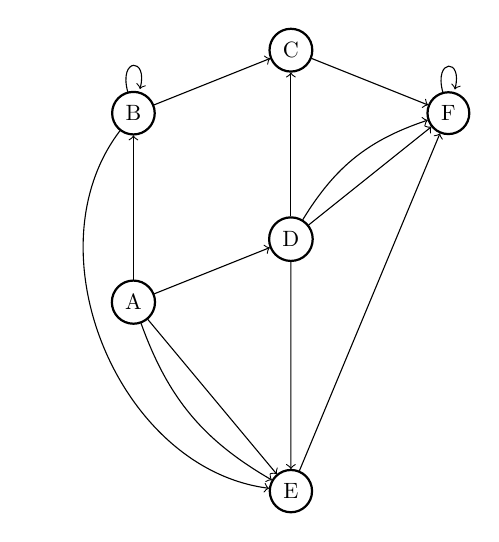
\begin{tikzpicture}[scale=0.8, transform shape]
	\begin{scope}[every node/.style={circle,thick,draw}]
		\node[] (A) at (0,0) {A};
    \node (B) at (0,3) {B};
    \node[] (C) at (2.5,4) {C};
		\node[] (D) at (2.5,1) {D};
    \node (E) at (2.5,-3) {E};
    \node (F) at (5,3) {F} ;
\end{scope}

\begin{scope}[
              every node/.style={fill=white,circle},
							every edge/.style={draw=black}]
							\path[->] (A) edge (B);
							\path[->] (B) edge (C);
							\path[->] (A) edge (D);
							\path[->] (D) edge (C);
							\path[->] (A) edge (E);
							\onslide<2>{\path[->] (A) edge[bend right=20] (E);}
							\path[->] (D) edge (E);
							\path[->] (D) edge (F);
							\onslide<2>{\path[->] (D) edge[bend left=20] (F);}
							\path[->] (C) edge (F);
							\path[->] (E) edge (F); 
							\path[->] (B) edge[bend right=60] (E); 
							\onslide<3>{\path[->] (B) edge[ loop above] (B);}
							\onslide<3>{\path[->] (F) edge[ loop above] (F);}
\end{scope}
\end{tikzpicture}

		\column{0.605\textwidth}
		\begin{itemize}
			\item A graph can also have a \textit{collection} of edges, rather than a set. We call this a \textit{multigraph}.
				\pause
			\item This allows multiple edges between the same pair of nodes.
				\pause
			\item Some versions also allow \textit{self-loops}.
				\pause
			\item But in our course we mostly consider \alert{simple} graphs, where $E$ is a set and there are no self-loops.
		\end{itemize}
	\end{columns}
\end{frame}

\begin{frame}
	\frametitle{Putting some edges together}
	\begin{columns}
		\column{0.405\textwidth}
			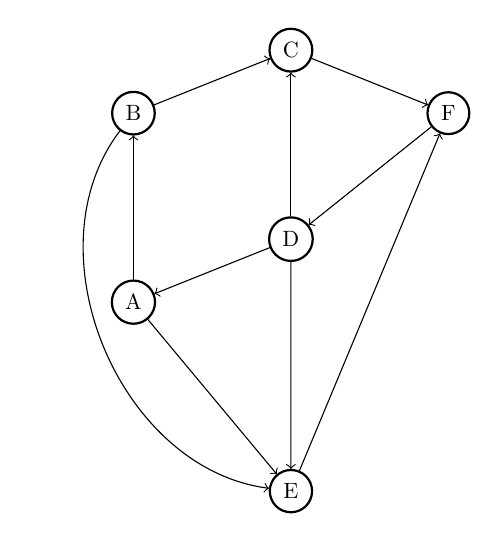
\begin{tikzpicture}[scale=0.8, transform shape]
	\begin{scope}[every node/.style={circle,thick,draw}]
		\node[] (A) at (0,0) {A};
    \node (B) at (0,3) {B};
    \node[] (C) at (2.5,4) {C};
		\node[] (D) at (2.5,1) {D};
    \node (E) at (2.5,-3) {E};
    \node (F) at (5,3) {F} ;
\end{scope}

\begin{scope}[
              every node/.style={fill=white,circle},
							every edge/.style={draw=black}]
							\path[->] (A) edge[] (B);
							\path[->] (B) edge[] (C);
							\path[->] (D) edge[] (A);
							\path[->] (D) edge (C);
							\path[->] (A) edge[] (E);
							\path[->] (D) edge (E);
							\path[->] (F) edge[] (D);
							\path[->] (C) edge[] (F);
							\path[->] (E) edge (F); 
							\path[->] (B) edge[bend right=60] (E); 
\end{scope}
\end{tikzpicture}

		\column{0.605\textwidth}
		\begin{itemize}
			\item A \textit{path} is a sequence of edges, connected to each other.
				\pause
			\item Paths can even contain the same nodes twice.
			\item The path in \alert{red} starts at $A$ and ends at $E$.
				\pause
			\item \textit{Cycles} are paths that start and end at the same vertex.
				\pause
			\item Simple paths and simple cycles allow every vertex at most once (with the exception for a cycle, where the
				starting vertex is equal to the ending vertex).
		\end{itemize}
	\end{columns}
\end{frame}

\begin{frame}
	\frametitle{Almost done!}
	\begin{block}{Paths}
		\begin{itemize}
			\item A path $\pi$ is commonly denoted as a sequence of vertices (in simple graphs), or a sequence of edges (in
				multi-graphs).
				\pause
			\item If denoted as a sequence of vertices, then $\pi$ is a path iff for every consecutive vertices $u,v$ in the
				sequence, $\{u,v\} \in E$.
				\pause
			\item If denoted as a sequence of edges, then $\pi$ is a path iff for every consecutive edges $e,f$ in the
				sequence, $e=\{u,v\}, f=\{v,w\}$ for some $u,v,w \in V$.
				\pause
			\item A cycle is a path $\pi = \{v_1, \dots, v_1\}$ (when denoted as a sequence of vertices).
				\pause
			\item For a directed graph, we can also speak of \textit{directed paths} and \textit{directed cycles}.
		\end{itemize}
	\end{block}	
\end{frame}

\begin{frame}
	\frametitle{The longest path}
	\begin{columns}
		\column{0.405\textwidth}
			\begin{tikzpicture}[scale=0.8, transform shape]
	\begin{scope}[every node/.style={circle,thick,draw}]
		\node[] (A) at (0,0) {A};
    \node (B) at (0,3) {B};
    \node[] (C) at (2.5,4) {C};
		\node[] (D) at (2.5,1) {D};
    \node (E) at (2.5,-3) {E};
    \node (F) at (5,3) {F} ;
\end{scope}

\begin{scope}[>={Stealth},
              every node/.style={fill=white,circle},
							every edge/.style={draw=black,very thick}]
							\path[->] (A) edge[onslide=<3>{draw=red}] (B);
							\path[->] (B) edge[onslide=<3>{draw=red}] (C);
							\path[->] (D) edge (A);
							\path[->] (D) edge (C);
							\path[->] (A) edge (E);
							\path[->] (D) edge[onslide=<3>{draw=red}] (E);
							\path[->] (F) edge[onslide=<3>{draw=red}] (D);
							\path[->] (C) edge[onslide=<3>{draw=red}] (F);
							\path[->] (E) edge (F); 
							\path[->] (B) edge[bend right=60] (E); 
\end{scope}
\end{tikzpicture}

		\column{0.605\textwidth}
		\begin{block}{Longest path?}
		\pause
			How many vertices are part of the longest simple path in this graph?
			\begin{enumerate}[A.]
				\item 4
				\item 5 
				\item 6
				\item 7
				\item I don't know.
			\end{enumerate}
		\end{block}
		\pause
		\vspace{-10pt}
		\begin{block}{All of them}
			In this case 6. \\
			Fun fact: this is actually a \alert{very very hard problem} that Computer Scientists cannot solve efficiently. More
			information on this when we discuss P vs NP.
		\end{block}
	\end{columns}
\end{frame}

\begin{frame}
	\frametitle{Finally we have reached the end}

		\begin{block}{Reachability}
			\begin{itemize}
				\item We say a node $v$ is \alert{reachable} from a node $u$ iff there is a (directed) path $\pi$ starting in
					$u$ and ending in $v$.
					\pause
				\item A directed graph is \alert{strongly connected} if for any two vertices there is a directed path between them.
				\item In other words, if $\forall u,v \in V:$ $v$ is reachable from $u$.
					\pause
				\item Finally then, a \alert{Directed Acyclic Graph (DAG)}  is a directed graph that has no cycles in it.
			\end{itemize}
		\end{block}	
\end{frame}

\begin{frame}
	\frametitle{DAG or $\neg$DAG}
	
	\begin{columns}
		\column{0.405\textwidth}
			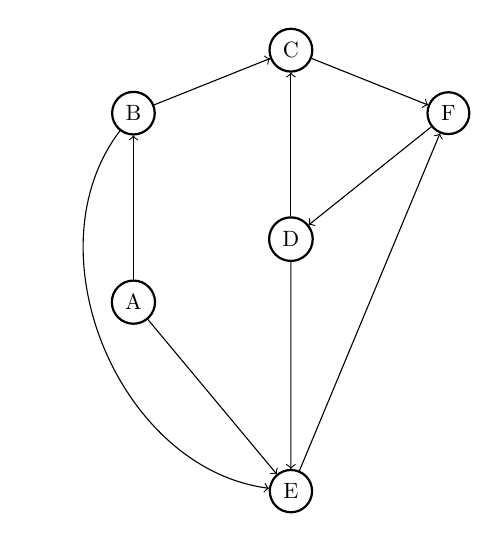
\begin{tikzpicture}[scale=0.8, transform shape]
	\begin{scope}[every node/.style={circle,thick,draw}]
		\node[] (A) at (0,0) {A};
    \node (B) at (0,3) {B};
    \node[] (C) at (2.5,4) {C};
		\node[] (D) at (2.5,1) {D};
    \node (E) at (2.5,-3) {E};
    \node (F) at (5,3) {F} ;
\end{scope}

\begin{scope}[
              every node/.style={fill=white,circle},
							every edge/.style={draw=black}]
							\path[->] (A) edge[] (B);
							\path[->] (B) edge[] (C);
							\path[->] (D) edge (C);
							\path[->] (A) edge (E);
							\path[->] (D) edge[] (E);
							\path[->] (F) edge[] (D);
							\path[->] (C) edge[] (F);
							\path[->] (E) edge (F); 
							\path[->] (B) edge[bend right=60] (E); 
\end{scope}
\end{tikzpicture}

		\column{0.605\textwidth}
		\begin{block}{Is this a DAG?}
		\pause
			Is this a DAG?
			\begin{enumerate}[A.]
				\item Yes
				\item No, but if we add one edge then it is.
				\item No, but if we remove one edge then it is.
				\item No, and we need to remove more than one edge to make it one.
				\item I don't know.
			\end{enumerate}
		\end{block}
		\pause
		\vspace{-10pt}
		\begin{block}{All of them}
			Just remove the edge $(F,D)$.
		\end{block}
	\end{columns}
\end{frame}


\begin{frame}
	\frametitle{Graph traversals}
	\framesubtitle{\scriptsize Image from \thinspace{\itshape Pixabay}}
	
	\begin{center}
		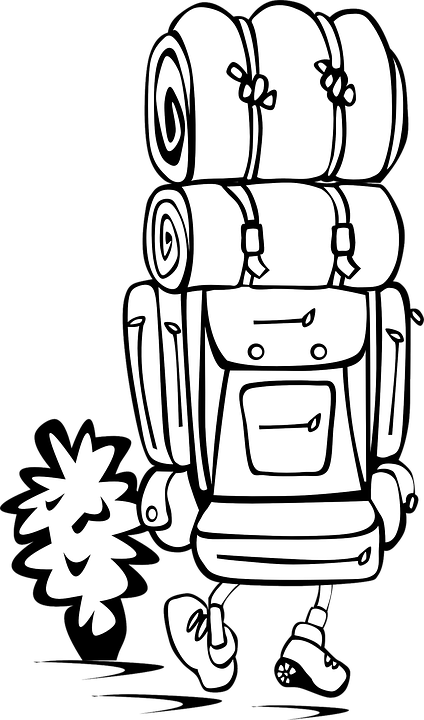
\includegraphics[width=0.3\textwidth]{images/backpacking.png}\\
		% https://pixabay.com/vectors/backpacking-backpacker-hiking-32069/
	\end{center}
\end{frame}

\begin{frame}
	\frametitle{Lets answer that first question!}

	\begin{block}{Can I get home?}
		Given the current state of the NS rail network, can I get home to Haarlem?
	\end{block}
	\pause
	\begin{block}{Search and ye shall find?}
		We can find out using a Breadth-first or Depth-first search.
	\end{block}
\end{frame}

\begin{frame}
	\frametitle{Depth-first Search}
	\framesubtitle{Recursion rules again}

		\begin{block}{DFS}
			Imagine you are walking in a labyrinth.\\
			\pause
			You bring a some paint and a piece of rope, tie it to the entrance and start walking. Here's what you do:\\
			\pause
			\begin{itemize}
				\item If we come to a cross-way, just pick one direction.
					\pause
				\item If we get to a dead-end, we back up to the last cross-way. Now use the paint to cross out the way you just
					went.
					\pause
				\item Repeat until you find the exit.
			\end{itemize}
		\end{block}	
	
\end{frame}

\begin{frame}
	\frametitle{An implementation}
	
	\begin{block}
		Function{DFS}{$v$}
	\pause
		For{each outgoing edge $e=(v,u)$ of $v$}
	\pause
		If{$u$ is not visited yet}
		State mark $u$ as visited
	\pause
		State Call{DFS}{$u$}
		EndIf
		EndFor
		EndFunction
		Comment{Ensure that $v$ is marked as visited before starting}
	\end{block}
	\pause
	\begin{columns}
		\column{0.455\textwidth}
	\begin{block}{Run time?}
		What is the run time of this algorithm?
		% \begin{multicols}{2}
		\begin{enumerate}[A.]
			\item $\Theta(|V|)$
			\item $\Theta(|E|)$
			\item $\Theta(|V| + |E|)$
			\item $\Theta(|V|\times|E|)$
		\end{enumerate}
	% \end{multicols}
	\end{block}
		\column{0.455\textwidth}
		\pause
		\begin{block}{}
			Worst-case we consider every vertex once and ever edge once.
		\end{block}
	\end{columns}
\end{frame}

\begin{frame}
	\frametitle{Let's apply it!}

	\begin{block}{Lets draw a graph}
		So lets draw a graph on the smart board and then apply DFS on it!
	\end{block}
\end{frame}

\begin{frame}
	\frametitle{But what if I don't like recursion\dots}
	\framesubtitle{Then tough luck! Don't worry, we got you covered!}

	\begin{block}{Getting rid of the recursion}
		How could we get rid of the recursion?
		\begin{enumerate}[A.]
			\item Adding nodes to explore to a set and taking the next node to visit randomly from the set.
			\item Adding nodes to explore to a stack and taking the next node to visit from the top of the stack.
			\item Adding nodes to explore to a queue and taking the next node to visit from the front of the queue.
			\item I don't know.
		\end{enumerate}
	\end{block}
\end{frame}

\begin{frame}
	\frametitle{An implementation}
	
	\begin{block}
		Function{DFS}{$v$}
		State $s gets$ empty Stack
		State $s$.push($v$)
		State mark $v$ as visited
		pause
		While{$s$ is not empty}
		State cur $gets$ $s$.pop()
		\pause
		For{each outgoing edge $e=(\text{cur},u)$ of $\text{cur}$}
		If{$u$ is not visited yet}
		State mark $u$ as visited
		\pause
		State $s$.push($u$)
		EndIf
		EndFor
		EndWhile
		EndFunction
	\end{block}
\end{frame}

\begin{frame}
	\frametitle{So what can we do with this?}

		\begin{block}{Many use cases!}
			\begin{itemize}
				\item Find a path between vertices, if one exists! (Including finding your way home to Haarlem.)\footnote{Try for
					yourself how you could reconstruct the path from the DFS. Or check page 645 of the book.}
					\pause
				\item Test if $G$ is a connected graph.
					\pause
				\item Find a cycle in $G$ if there is one (that $v$ is a part of).
			\end{itemize}
			
		\end{block}	
\end{frame}

\begin{frame}
	\frametitle{What if we use a queue though?}
	
	\pause
	\begin{block}
		Function{BFS}{$v$}
		State $s gets$ empty \alert{Queue}
		State $s$.enqueue($v$)
		State mark $v$ as visited
		While{$s$ is not empty}
		State cur $gets$ $s$.dequeue()
		For{each outgoing edge $e=(\text{cur},u)$ of $\text{cur}$}
		If{$u$ is not visited yet}
		State mark $u$ as visited
		State $s$.enqueue($u$)
		EndIf
		EndFor
		EndWhile
		EndFunction
	\end{block}
\end{frame}
	
\begin{frame}
	\frametitle{So what does this BFS do?}

		\begin{block}{BFS}
			We crawl over the graph, layer by layer.\\
			\pause
			First we check all vertices at distance $1$ from our starting point.\\
			\pause
			Then all vertices at distance $2$.\\
			Etc. Etc.
		\end{block}	
	\begin{block}{Lets draw a graph}
		So lets draw a graph on the smart board and then apply BFS on it!
	\end{block}
\pause
	
\end{frame}


\begin{frame}
	\frametitle{Topological Ordering}
	
	\begin{center}
		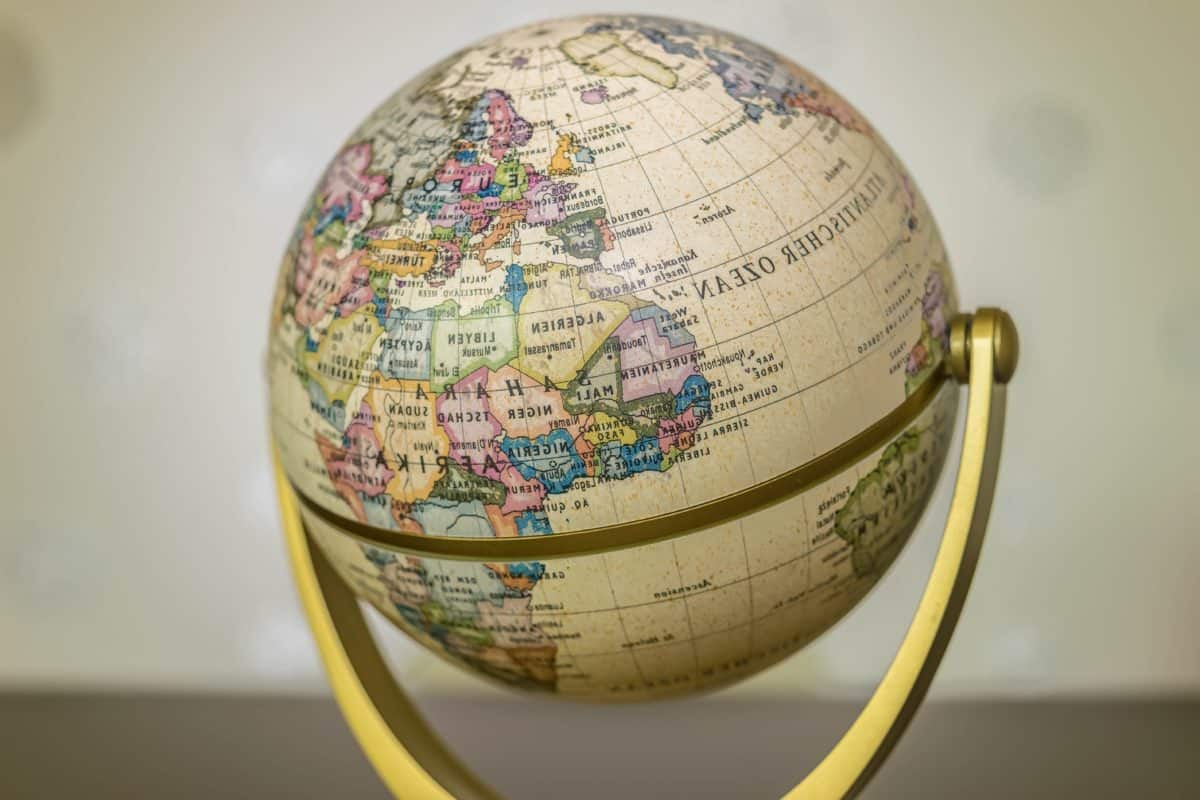
\includegraphics[width=0.68\textwidth]{images/topology.jpeg}\\
		\hspace*{15pt}\hbox{\scriptsize Image By:\thinspace{\itshape Tama66}}
		% https://pixnio.com/objects/geography-map-earth-globe-object-education-topology#
	\end{center}
\end{frame}

\begin{frame}
	\frametitle{Jobs to do!}
	\framesubtitle{Remember we saw this as a use case of the pre-order traversal in the binary tree.}
	\begin{block}{Tons of things to do}
		I have a bunch of things to do, that depend on each other. My question is, what order can I do them in so that all
		dependencies are met?
	\end{block}
	\pause
	\begin{columns}
		\column{0.455\textwidth}
		\begin{block}{For example...}
			I need to do the following things:
			\begin{itemize}
				\item Create an exam
		\pause
				\item Have the exam proof read
				\item Print the exam
		\pause
				\item Make the answer sheet
				\item Print the answer sheet
		\pause
				\item Bring everything to location
			\end{itemize}
		\end{block}	
		\column{0.455\textwidth}
		\pause
			\begin{block}{Lets draw that}
				Lets make that into a graph!\\
				Tasks become vertices.\\
				And dependencies become edges.\\
			\end{block}	
	\end{columns}
\end{frame}

\begin{frame}
	\frametitle{Now what do we need?}
	
		\begin{block}{A topological ordering}
			A topological ordering of the vertices $V$ in a \textit{directed} graph, is an ordering $v_1, \dots, v_n$ such
			that $e=(v_i,v_j)$ with $i < j$ for all $e \in E$.
		\end{block}	

		\pause
		\begin{block}{DAGs and topological orderings}
			A graph $G$ has a topological ordering if and only if it is a DAG.
		\end{block}	
		\pause
		\begin{proof}
			(first part) Suppose $G$ has a topological ordering.\\
			\pause
			We now use a proof by contradiction. Assume there is a cycle (i.e. it is no DAG). That means there is a cycle
			$(v_x, v_y), \dots (v_w, v_x)$. But if it has a topological ordering, then $x < y < w < x$, which is clearly not
			possible.\\
			\pause
			(second part) A little harder... Let's make an algorithm!
		\end{proof}
\end{frame}

\begin{frame}
	\frametitle{The idea}
	\begin{overlayarea}{\textwidth}{\textheight}
		\begin{block}{The idea}
			\begin{itemize}
				\item 
					If $G$ is acyclic, there must be some vertex without incoming edges.\\
				\item<3->
					We can start with this one, add it to the topological ordering and remove its outgoing edges.\\
				\item<4->
					Now repeat!
			\end{itemize}
		\end{block}	
		\only<2>{
			\begin{block}{Why?}
				Why must this be the case?
			\end{block}
		}
	\end{overlayarea}
\end{frame}

\begin{frame}
	\frametitle{Lets code it!}
	
	\begin{columns}
		\column{0.555\textwidth}
		{
	\small
	\begin{block}
		Function{Topo}{$G$}
		State order $gets$ empty list
		State q $gets$ empty queue
		\pause
		State $v gets$ a random vertex with $\mathit{indeg}(v) = 0$.
		State q.enqueue($v$)
		\pause
		While{q is not empty}
		State $v gets$ q.dequeue()
		State order.append($v$)
		\pause
		For{each outgoing edge $e=(v,u)$ of $v$}
		State $G$.remove(e)
		\pause
		If{$\mathit{indeg}(u) == 0$}
		State q.enqueue($u$)
		\pause
		EndIf
		EndFor
		EndWhile
		EndFunction
	\end{block}
}
			
		\column{0.405\textwidth}
			\begin{block}{Run time}
				\begin{itemize}
					\item If we implement this efficiently\dots
						\pause
					\item Then finding the first vertex is $\Theta(|V|)$
						\pause
					\item We then consider all vertices at most once: $\Theta(|V|)$
						\pause
					\item We also remove all edges at most once (which our map-based implementation can do in expected
						$\Theta(1)$): $\Theta(|E|)$.
					\item All-in-all: $\Theta(|V| + |E|)$.
				\end{itemize}	
			\end{block}	
			
	\end{columns}
\end{frame}

\begin{frame}
	\frametitle{One closing remark}
	
		\begin{block}{One important difference}
			Both DFS/BFS and the topological ordering give an order of the nodes.\\
			\pause
			But is there a difference? (Other than the order in which they are returned?)
		\end{block}	

		\pause
		\begin{block}{Yes!}
			DFS/BFS require a starting node! And give different results (not necessarily the whole graph) when starting from
			different nodes.\\
			\pause
			Topological orderings are Graph properties, not depending on a specific vertex!
		\end{block}
\end{frame}

\begin{frame}
	\frametitle{Implementing a graph}

	\begin{block}{Implementations}
		There are many options:
		\begin{itemize}
			\item Edge List: just keep one list of all edges of the graph.
				\pause
			\item Adjacency List: for every vertex, keep a list of all incident edges.
				\pause
			\item Adjacency Matrix: a massive 2D array of size $|V|\times |V|$. Every entry can hold an edge.
				\pause
			\item Adjacency Map: Just the best option. We will discuss this one now.
		\end{itemize}
	\end{block}	
\end{frame}

\begin{frame}
	\frametitle{Vertex class}
	
	\begin{columns}
		\column{0.505\textwidth}
			\lstinputlisting[basicstyle=\tiny\ttfamily, 
			% linebackgroundcolor={%
			% \btLstHL<2>{3-5}%
			% \btLstHL<3>{7-8}%
			% \btLstHL<4>{10-11}%
			% \btLstHL<5>{13-15}%
			% \btLstHL<6>{17-23}%
			% },
			lastline=23
			]{src/vertex.py}
		\column{0.455\textwidth}
		\begin{itemize}
			\pause
			\item Initialise a Vertex, with a \texttt{dict} to hold neighbours.
				\pause
			\item It is now $O(1)$ to add an edge, but this only works for \textit{simple} graphs.
				\pause
			\item Getting all neighbours is $O(\mathit{deg}(v))$, which is the best we can get.
				\pause
			\item A generator that allows us to iterate over the (outgoing) edges of this node.
				\pause
			\item And we can make more functions as need be.
		\end{itemize}
			
	\end{columns}
\end{frame}

\begin{frame}
	\frametitle{Graph class}
	
	\begin{columns}
		\column{0.505\textwidth}
			\lstinputlisting[basicstyle=\tiny\ttfamily, 
			% linebackgroundcolor={%
			% \btLstHL<2>{3-4}%
			% \btLstHL<3>{6-7}%
			% \btLstHL<4>{9-10}%
			% },
			lastline=10
			]{src/graph.py}
		\column{0.455\textwidth}
		\begin{itemize}
			\pause
			\item A graph is just a bunch of vertices now.
				\pause
			\item Adding a vertex is adding it to the dictionary.
			\item Using a dictionary allows $O(1)$ retrieval based on node name (e.g.\ Amsterdam)
				\pause
			\item Getting all vertices, is just all values from the list.
		\end{itemize}
			
	\end{columns}
\end{frame}

\begin{frame}
	\frametitle{Graphs are everywhere!}
	
	\begin{center}
		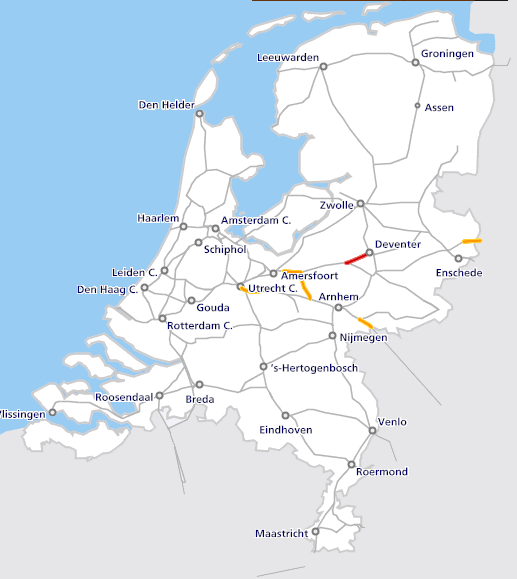
\includegraphics[width=0.35\textwidth]{images/ns.png}\\
		\hspace*{15pt}\hbox{\scriptsize Screenshot by: \thinspace{\itshape Stefan Hugtenburg}}\\
		\hspace*{15pt}\hbox{\scriptsize Taken from: \url{https://ns.nl}}
	\end{center}
\end{frame}

\begin{frame}
	\frametitle{Rail networks}
	
	\begin{overlayarea}{\textwidth}{\textheight}
			\begin{block}{Questions to ask}
				The NS maintains a large network of railroads in the Netherlands. There are many questions related to this:
				\begin{itemize}
					\item \alert<5>{What cities can you reach by train?}
						\pause
					\item \alert<6>{What is the quickest way to get from A to B?}
						\pause
					\item \alert<7>{What is the best way to connect new stations to the network?}
						\pause
					\item \alert<8>{How can we quickly tour the entire country?}
				\end{itemize}
			\end{block}
			\only<5>{
			\begin{block}{Traversals}
				This we can figure out by traversing the graph, which we will do today.
			\end{block}
		}
		\only<6>{
			\begin{block}{Shortest path algorithms}
				This we can figure out by using a shortest path algorithm (next Monday).
			\end{block}
		}
		\only<7>{
			\begin{block}{Shortest path algorithms}
				This we can figure out by using a Minimum Spanning Tree (next Tuesday).
			\end{block}
		}
		\only<8>{
			\begin{block}{TSP}
				This we cannot figure out! It's called the Travelling Salesman Problem (Monday two weeks from now)
			\end{block}
		}
	\end{overlayarea}
\end{frame}

\begin{frame}
	\frametitle{Summary}

		\begin{block}{This implementation is awesome!}
			This implementation is better than all others (that you can find in the book), tomorrow we will see to what extent you can
			reproduce these ideas in the tutorial.
		\end{block}	

		\pause
		\begin{tabular}{c | c}
		Operation & Time complexity \\
		\midrule
		$|V|$ & $\Theta(1)$ \\
		$|E|$ & $\Theta(|V|)$\footnote{But we could make this $\Theta(1)$} \\
		\pause
		\texttt{degree(v)} & $\Theta(1)$ \\
		\texttt{neighbours(v)} & $\Theta(\mathit{deg}(v))$ \\
		\pause
		\texttt{add\_vertex(v)} & $\Theta(1)$ \\
		\texttt{add\_edge(v)} & $\Theta(1)$ \\
		\pause
		And a bunch more & See the book if you want\\
		\end{tabular}
\end{frame}

